\documentclass[../Master.tex]{subfiles}
\begin{document}
\chapter{Experimental section}\label{cha:experimental-section}
\section{Dimethyl 4,4'-malonyldibenzoate}
\subsection{Synthesis}

\begin{center}
	\begin{tabular}[b]{lccccccc}
		\toprule
		Reagent                 & CAS       & MW / \(g \ mol^{-1}\) & m / g & n / mmol & SR   \\
		\midrule
		methyl 4-acetylbenzoate & 3609-53-8 & 178.19                & 4.400 & 24.69    & 1.20 \\
		dimethyl terephthalate  & 120-61-6  & 194.19                & 4.000 & 20.60    & 1.00 \\
		NaH, mineral dispersion & 7646-69-7 & 23.998                & 1.132 & 47.17    & 2.30 \\
		\bottomrule
	\end{tabular}
\end{center}

The reaction is carried out under N$_{2}$ atmosphere, the reactant are carefully dried beforehand.\\
In a flask, 1.132 g of NaH dispersion in mineral oil are washed with anhydrous THF (15 mL x 2).\\
4.0 g of methyl 4-acetyl benzoate and 4.4 g of dimethyl terephthalate are dissolved in 45 mL of anhydrous THF, and then NaH suspension in THF is added.\\
The mixture is heated to reflux overnight. \\
Evaporation of the solvent under vacuum gives a dark brown compound. The solid is taken up in water and acidified with HCl 20\% in an ice bath. Taking care to leave it to react for a few hours and checking the pH to make sure it is acid. More water is added if mixing is particularly difficult.\\
The raw product is recovered as a yellow solid by filtration with a Buchner funnel.
To eliminate the impurities of the remaining reagents the solid is washed with chloroform and with diethyl ether. The solid is lastly collected on a Buchner funnel and dried. Yield: 92\%, 8.67 g of product.

\newpage
\subsection{Characterization}

\subsubsection{NMR}
\begin{figure}[h!]
	\centering
	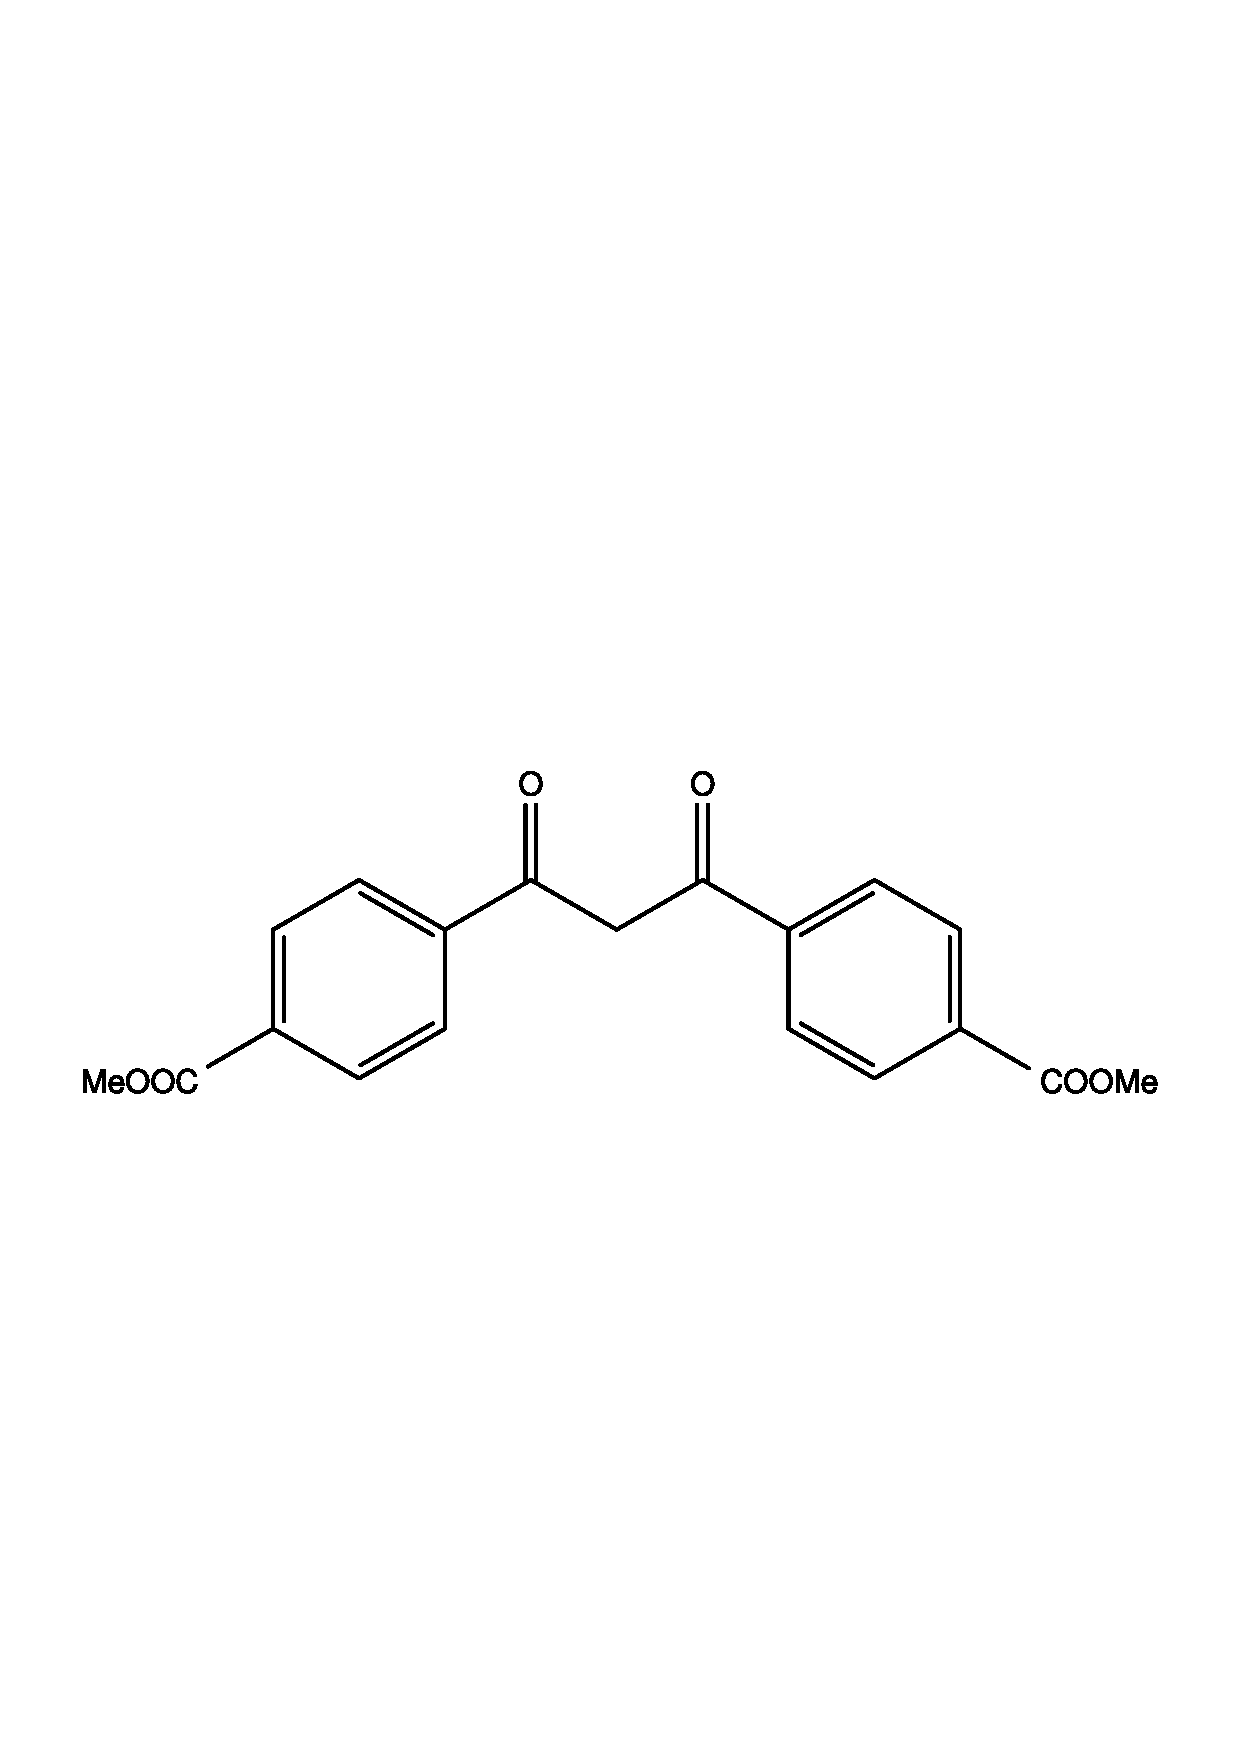
\includegraphics[width=12cm,keepaspectratio]{Spectra/nmr/dikest2.pdf}
\end{figure}
\begin{figure}[h!]
	\centering
	\includegraphics[width=12cm,keepaspectratio]{Spectra/nmr/dikest.pdf}
\end{figure}

\subsubsection{IR}

% TODO: aggiungere ir dell'estere di simo

\newpage
\section{4,4'-malonyldibenzoic acid}
\subsection{Synthesis}

\begin{center}
	\begin{tabular}[b]{lccccccc}
		\toprule
		Reagent                         & CAS       & MW / \(g \ mol^{-1}\) & m / g & n / mmol & SR \\
		\midrule
		Dimethyl 4,4'-malonyldibenzoate & -         & 340.31                & 1.000 & 2.940    & 1  \\
		LiOH                            & 1310-65-2 & 23.95                 & 1.411 & 58.80    & 20 \\
		\bottomrule
	\end{tabular}
\end{center}

In a small beaker, 1.411 g of freshly ground LiOH is dissolved in 10 mL of water. In an flask, 1.000 g of 4,4'-malonyldibenzoate is suspended in 10 mL of THF, then the LiOH solution is slowly added. The mixture is allowed to react 7 hours at room temperature under vigorous stirring. It is then proceeded by extracting with \(CHCl_{3}\) (3x25 mL). The aqueous phase is collected and acidified with 10 \% HCl to acidic pH, observing the formation of straw-yellow precipitate. The solid is recovered by filtration over buchner and allowed to air dry.

\newpage
\subsection{Characterization}
\subsubsection{NMR}

% TODO: aggiungere nmr dell'acido di simo

\subsubsection{IR}

% TODO: aggiungere ir dell'acido di simo

\newpage
\section{Methyl 4,4'-(1H-pyrazole-3,5-diyl)dibenzoate}
\subsection{Synthesis from methyl 4,4'malonyldibenzoate}
\subsubsection{EtOH}
A typical synthesis is described here:
500 mg of dimethyl 4,4'-malonyldibenzoate is suspended in 20 mL of EtOH in a 50 mL flask. The mixture is left in ultrasonic bath for 30'. 350 \(\mu L\) of hydrazine monohydrate are slowly added to the mixture that is then heated to reflux overnight.\\
The compound is collected as a pale yellow solid on a teflon funnel. Yield: 25\%.
\subsubsection{DMF}
500 mg of dimethyl 4,4'-malonyldibenzoate is suspended in 15 mL of DMF in a 50 mL flask. The mixture is left in ultrasonic bath for 30'. 350 \(\mu L\) of hydrazine monohydrate are slowly added to the mixture that is then heated to 150°C overnight.\\
Evaporation of the solvent under vacuum gives a white ivory solid. The compound is then washed adding 25 mL of ethanol and heat to reflux for 2 hours. Pure solid is collected on a Buchner funnel. Yield: 48\%.
\subsubsection{DMSO}
500 mg of dimethyl 4,4'-malonyldibenzoate is solubilized in 20 mL of DMSO in a 50 mL flask. The mixture is left in ultrasonic bath for 30'. 350 \(\mu L\) of hydrazine monohydrate are slowly added to the mixture that is then heated to 150°C overnight.\\
\pagebreak
\subsubsection{Characterization}
\newline
\paragraph{NMR}

% TODO: aggiungere nmr del pirazolo estere

\paragraph{IR}

% TODO: aggiungere IR del pirazolo estere

\newpage \subsection{Synthesis from \\Methyl 4-[(1E)-3-[4- (methoxycarbonyl) phenyl]-3-oxoprop-1-en-
1-yl]benzoate}

\paragraph{Acetic acid}

\begin{center}
	\begin{tabular}[b]{lccccccc}
		\toprule
		Reagent               & CAS       & MW / \(g \ mol^{-1}\) & m / g & n / mmol & SR \\
		\midrule
		Unsaturated compound  & -         & 324.332               & 0.370 & 1.14     & 1  \\
		\(N_2H_4 \cdot H_2O\) & 7803-57-8 & 50.05                 & 0.166 & 3.42     & 3  \\
		\bottomrule
	\end{tabular}
\end{center}

%  Si disperde ***SM51*** in acido acetico, si pone sotto forte agitazione,
% aggiungendo lentamente idrazina. Si lascia reagire a temperatura ambiente, dopo
% circa un'ora non si osserva formazione di precipitato. La miscela di reazione
% viene scaldata fino a 90°, si osserva la dissoluzione di ***SM51***, soluzione
% di colore giallo scuro. % Si lascia reagire per altre 3 ore. Si procede
% raffreddatto la miscela in frigo, nonostante quanto atteso non si osserva
% precipitazione. Si aggiunge acqua fredda e si osserva precipitazione, si filtra
% e si lascia asciugare. % Verificando all'NMR si osserva la presenza di una
% piccola parte di pirazolo e in gran parte del reagente iniziale. Per questo il
% solido viene ripreso nelle stesse condizioni iniziali (aggiunta alcune gocce di
% solforico) e rimesso a reagire. Si mette direttamente la temperatura a 120 gradi
% (reflusso dell'acido acetico). A differenza della prima reazione non si osserva
% solubilizzazione completa.

\paragraph{EtOH with HCl}

\begin{center}
	\begin{tabular}[b]{lccccccc}
		\toprule
		Reagent               & CAS       & MW / \(g \ mol^{-1}\) & m / g & n / mmol & SR \\
		\midrule
		Unsaturated compound  & -         & 324.332               & 0.300 & 0.92     & 1  \\
		\(N_2H_4 \cdot H_2O\) & 7803-57-8 & 50.05                 & 0.138 & 2.76     & 3  \\
		\bottomrule
	\end{tabular}
\end{center}

% ***SM56*** viene sospeso in 5 mL di metanolo con 20% di acido cloridrico, la
% solubilizzazione é fortemente esotermica. Si procede all'aggiunta di idrazina
% molto lentamente, che provoca una violenta reazione (che ci si aspettava
% considerata l'aciditá della slz). La miscela viene portata a reflusso, dopo
% circa due ore non si osserva alcun cambiamento. Il reagente non reagito viene
% recuperato per filtrazione, e viene recuperato. Lo stesso reagente viene rimesso
% a reagire in assenza di catalizzatore a reflusso per circa 5 ore. Prima di
% osservare la formazione di prodotto biancastro con fotolumiscenza nel blu si
% osserva la formazione di un intermedio giallo non solubile, che gradualmente
% torna in soluzione, questo potrebbe essere l'intermedio idrazonico. Considerato
% quanto svolto prima di ottenere un precipitato si decide di rimettere la prova a
% partire da zero ***SM60***.


\paragraph{EtOH with pyridine}

\begin{center}
	\begin{tabular}[b]{lccccccc}
		\toprule
		Reagent               & CAS       & MW / \(g \ mol^{-1}\) & m / g & n / mmol & SR \\
		\midrule
		Unsaturated compound  & -         & 324.332               & 0.300 & 0.92     & 1  \\
		\(N_2H_4 \cdot H_2O\) & 7803-57-8 & 50.05                 & 0.138 & 2.76     & 3  \\
		\bottomrule
	\end{tabular}
\end{center}

%  ***SM56*** viene sospeso in 10 mL di metanolo con 20% di pyridina (anche se
% quest'ultima disponibile in laboratorio possiede un colore marrone, poco consono
% visto che la piridina dovrebbe essere incolore). Si aggiunge lentamente idrazina
% e si porta a reflusso, dopo pochi minuti i reagenti si solubilizzano
% completamente e osservando con la lampada si osserva fotolumiscenza nel blu.
% Tuttavia non si osserva formazione di molto precipitato, neanche dopo
% raffreddamento in frigo. Il poco precipitato viene comunque recuperato e si
% conduce un NMR per verificare.


\paragraph{EtOH}

\begin{center}
	\begin{tabular}[b]{lccccccc}
		\toprule
		Reagent               & CAS       & MW / \(g \ mol^{-1}\) & m / g & n / mmol & SR \\
		\midrule
		Unsaturated compound  & -         & 324.332               & 0.500 & 1.54     & 1  \\
		\(N_2H_4 \cdot H_2O\) & 7803-57-8 & 50.05                 & 0.231 & 4.62     & 3  \\
		\bottomrule
	\end{tabular}
\end{center}

% TODO: aggiungere descrizione della procedura
% 500 mg di composto ***SM59*** vengono dispersi in 10 mL di metanolo, viene
% aggiunta lentamente l'idrazina e si lascia reagire overnight. Questa prova
% permetterá di valutare meglio la risposta alle condizioni che sembrano aver
% portato a buoni risultati in ***SM60***. In seguito all'NMR condotto su
% ***SM60*** la miscela di reazione viene portata a reflusso per circa 5h. Viene
% lasciata raffreddare molto lentamente, lasciando il pallone a filo dell'olio. Si
% osserva la formazione di precipitato cristallino, che viene filtrato e lasciato
% asciugare. Su questo sará necessaria condurre NMR per verificare se é stata
% completata la trasformazione. Si nota inoltre che il prodotto restituisce
% fotolumiscenza nel blu anche con la lampada disponibile in laboratorio, a
% differenza di ***SM60***. L'NMR


\newpage \subsection{Characterization}
\subsubsection{NMR}
\subsubsection{IR}

\newpage \section{4,4'-(1H-pyrazole-3,5-diyl)dibenzoic acid}
\subsection{Synthesis}
\subsubsection{LiOH}
\begin{center}
	\begin{tabular}[b]{lccccccc}
		\toprule
		Reagent                                   & CAS       & MW / \(g \ mol^{-1}\) & m / g  & n / mmol & SR \\
		\midrule
		4,4'-(1H-pyrazole-3,5-diyl)dibenzoic acid & -         & 336.47                & 0.3023 & 0.8988   & 1  \\
		LiOH                                      & 1310-65-2 & 23.95                 & 0.4505 & 17.796   & 20 \\
		\bottomrule
	\end{tabular}
\end{center}

In a small beaker, 0.4505 g of freshly ground LiOH is dissolved in 6 mL of water. In an flask, 0.3023 g of methyl 4,4'-(1H-pyrazole-3,5-diyl)dibenzoate is suspended in 6 mL of THF, then the LiOH solution is slowly added. The mixture is allowed to react overnight at room temperature under vigorous stirring. It is then proceeded by extracting with \(CHCl_{3}\) (3x25 mL). The aqueous phase is collected and acidified with 10 \% HCl to acidic pH, observing the formation of white precipitate. The solid is recovered by filtration over buchner and allowed to air dry.

\newpage \subsection{Characterization}
\subsubsection{NMR}

% TODO: manca nmr del pirazolo acido

\subsubsection{IR}

% TODO: manca ir del pirazolo acido

\newpage \section{4,4'-malonyldibenzonitrile}
\subsection{Synthesis}
\begin{center}
	\begin{tabular}[b]{cccccccc}
		\toprule
		Reagent                & CAS       & MW / \(g \ mol^{-1}\) & m / g  & n / mmol & SR   \\
		\midrule
		methyl 4-cyanobenzoate & 1129-35-7 & 161.16                & 4.0370 & 25.05    & 0.93 \\
		4-acetylbenzonitrile   & 1443-80-7 & 145.16                & 3.3862 & 23.32    & 1.00 \\
		NaH                    & 7646-69-7 & 23.998                & 2.7780 & 115.75   & 4.96 \\
		\bottomrule
	\end{tabular}
\end{center}
The reaction is carried out under N$_{2}$ atmosphere, the reactant are carefully dried beforehand.\\
In a flask, 2.778 g of NaH dispersion in mineral oil are washed with anhydrous THF (15 mL x 2).\\
4.0370 g of methyl 4-cyanobenzoate and 3.3862 g of 4-acetylbenzonitrile are dissolved in 45 mL of anhydrous THF, and then NaH suspension in THF is added under ice bath while vigouros mixing. \\
The mixture is allowed to reach room temperature and then is heated to reflux overnight. \\
Evaporation of the solvent under vacuum gives a dark green compound. The solid is taken up in water and acidified with HCl 20\% in an ice bath. Taking care to leave it to react for a few hours and checking the pH to make sure it is acid. More water is added if mixing is particularly difficult.\\
The raw product is recovered as a yellow solid by filtration with a Buchner funnel.
To eliminate the impurities of the remaining reagents the solid is washed with ethanol. The solid is lastly collected on a Buchner funnel and dried. Yield: 74\%, 4.76 g of product.
\pagebreak

\subsection{Characterization}
\subsubsection{NMR}
\begin{figure}[h!]
	\centering
	\includegraphics[width=12cm,keepaspectratio]{Spectra/nmr/dicn.pdf}
	\caption{DikDiCN \NMR*(400)}
\end{figure}
\begin{figure}[h!]
	\centering
	\includegraphics[width=12cm,keepaspectratio]{Spectra/nmr/dicn2.pdf}
	\caption{DikDiCN \NMR*(400), zoom on diagonistic peaks}
\end{figure}
\newpage
\section{Methyl 4‐[(1E)‐3‐[4‐(methoxycarbonyl)phenyl]‐3‐oxoprop‐1‐en‐1‐yl]benzoate}
\subsection{Synthesis}
\begin{center}
	\begin{tabular}[b]{cccccccc}
		\toprule
		Reagent                 & CAS       & MW / \(g \ mol^{-1}\) & m / g & n / mmol & SR  \\
		\midrule
		methyl 4‐formylbenzoate & 1571-08-0 & 178.18                & 0.500 & 2.8      & 1   \\
		methyl 4‐acetylbenzoate & 3609-53-8 & 164.16                & 0.550 & 3.5      & 1.2 \\
		NaOH                    & 1310-73-2 & 39.998                & 0.230 & 5.6      & 2   \\
		\bottomrule
	\end{tabular}
\end{center}

In a small beaker, 230 mg of freshly ground NaOH is dissolved in 10 mL of methanol. \\
In a flask, 500 mg methyl 4-formylbenzoate and 550 mg methyl 4-acetylbenzoate are dissolved in 5 mL MeOH. The mixture is placed under vigorous stirring in an ice bath. The freshly prepared sodium hydroxide solution is slowly added. The reaction is left to react overnight. \\
The yellowish solid is collected on Buchner funnel and allowed to air dry. Yield 94\%, 0.85 g of product.

\subsection{Characterization}
\subsubsection{NMR}

\begin{figure}[h!]
	\centering
	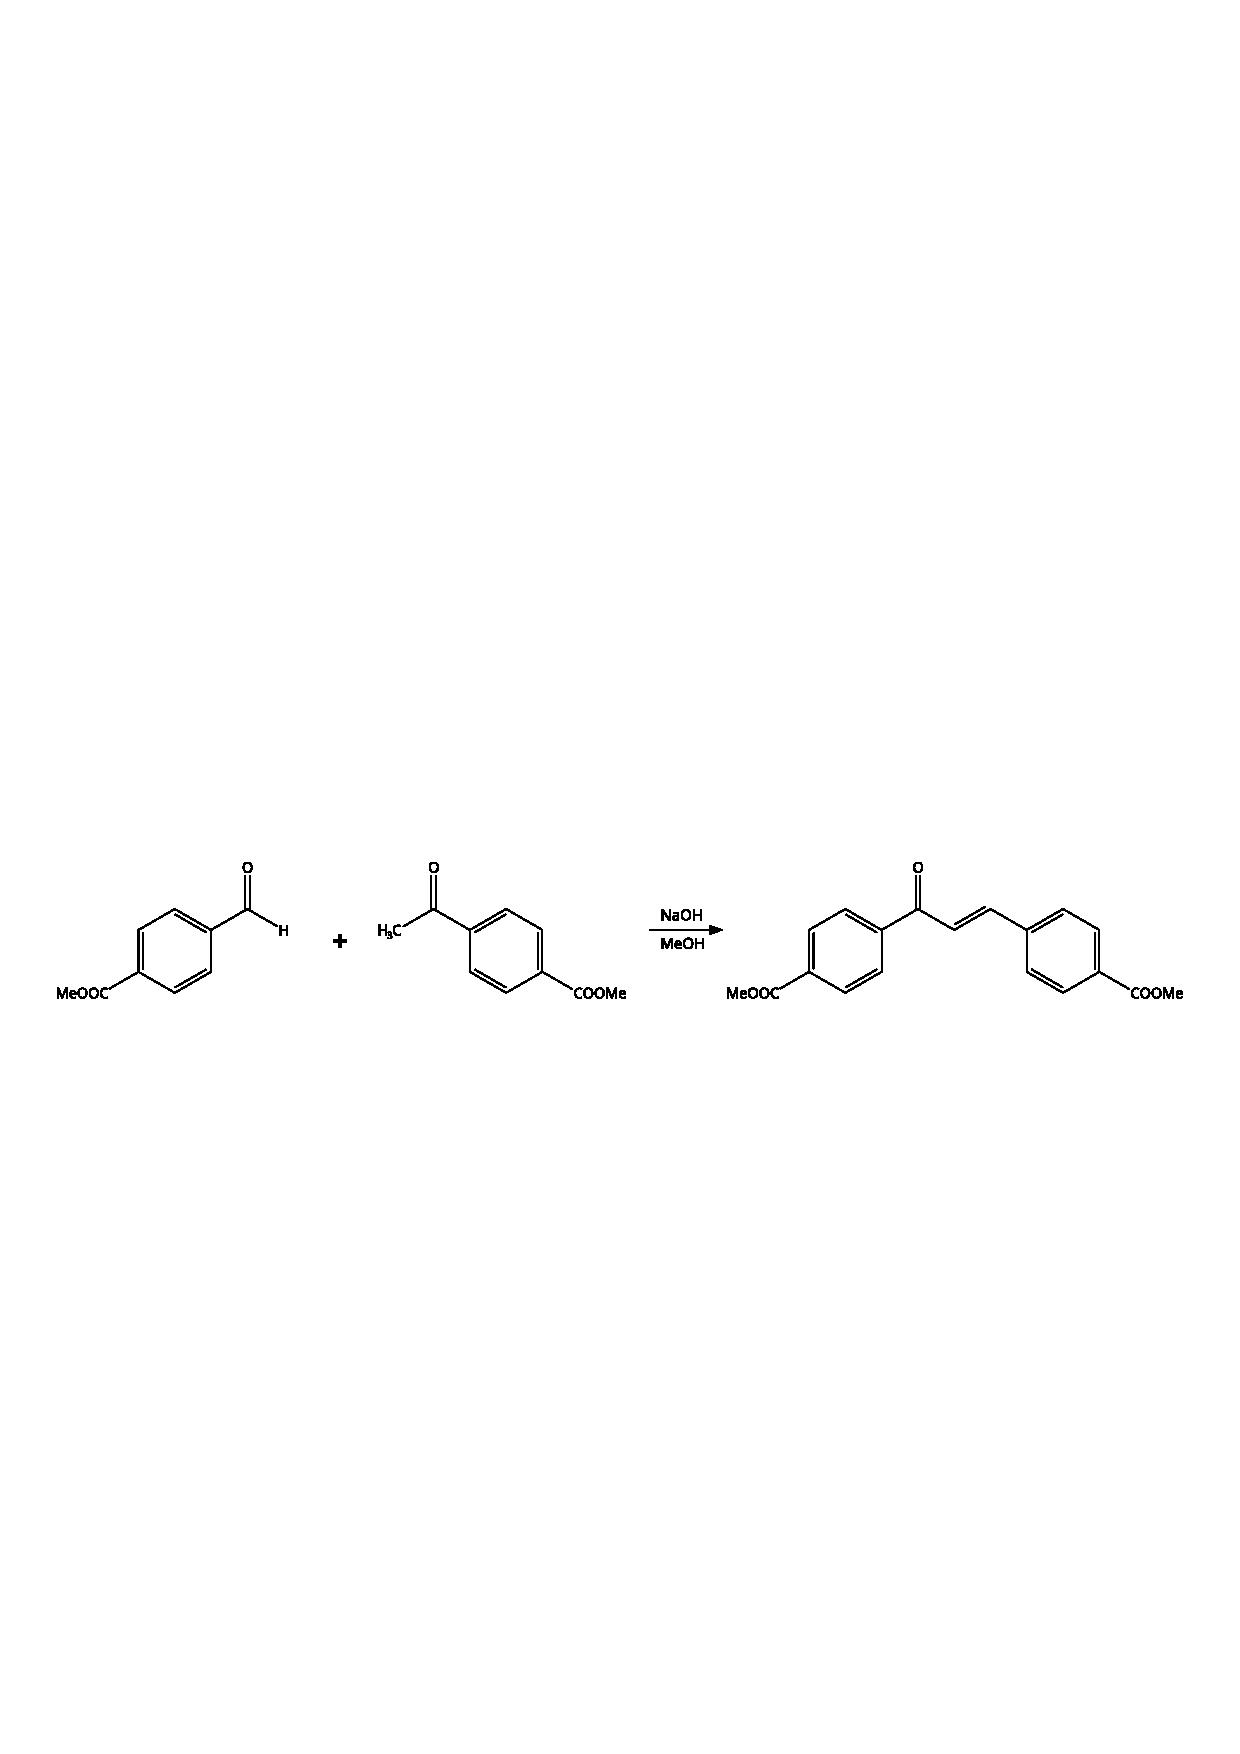
\includegraphics[width=12cm,keepaspectratio]{Spectra/nmr/aldolica.pdf}
	\caption{HNMR}
\end{figure}

\begin{figure}[h!]
	\centering
	\includegraphics[width=12cm,keepaspectratio]{Spectra/nmr/aldolica2.pdf}
	\caption{HNMR zoom}
\end{figure}

\end{document}
%%% Local Variables:
%%% mode: latex
%%% TeX-master: "../Master"
%%% End:

